%%%%%%%%%%%%%%%%%%%%%%%%%%%%%%%%%%%%%%%%%
% Short Sectioned Assignment
% LaTeX Template
% Version 1.0 (5/5/12)
%
% This template has been downloaded from:
% http://www.LaTeXTemplates.com
%
% Original author:
% Frits Wenneker (http://www.howtotex.com)
%
% License:
% CC BY-NC-SA 3.0 (http://creativecommons.org/licenses/by-nc-sa/3.0/)
%
%%%%%%%%%%%%%%%%%%%%%%%%%%%%%%%%%%%%%%%%%

%----------------------------------------------------------------------------------------
%	PACKAGES AND OTHER DOCUMENT CONFIGURATIONS
%----------------------------------------------------------------------------------------

\documentclass[paper=a4, fontsize=11pt]{scrartcl} % A4 paper and 11pt font size
\usepackage[margin=0.7in]{geometry}
\usepackage[T1]{fontenc} % Use 8-bit encoding that has 256 glyphs
\usepackage{fourier} % Use the Adobe Utopia font for the document - comment this line to return to the LaTeX default
\usepackage[english]{babel} % English language/hyphenation
\usepackage{amsmath,amsfonts,amsthm} % Math packages

\usepackage{lipsum} % Used for inserting dummy 'Lorem ipsum' text into the template

\usepackage{sectsty} % Allows customizing section commands
\allsectionsfont{\normalfont\scshape} % Make all sections centered, the default font and small caps

\usepackage{fancyhdr} % Custom headers and footers
\pagestyle{fancyplain} % Makes all pages in the document conform to the custom headers and footers
\fancyhead{} % No page header - if you want one, create it in the same way as the footers below
\fancyfoot[L]{} % Empty left footer
\fancyfoot[C]{} % Empty center footer
\fancyfoot[R]{\thepage} % Page numbering for right footer
\renewcommand{\headrulewidth}{0pt} % Remove header underlines
\renewcommand{\footrulewidth}{0pt} % Remove footer underlines
\setlength{\headheight}{13.6pt} % Customize the height of the header

\numberwithin{equation}{section} % Number equations within sections (i.e. 1.1, 1.2, 2.1, 2.2 instead of 1, 2, 3, 4)
\numberwithin{figure}{section} % Number figures within sections (i.e. 1.1, 1.2, 2.1, 2.2 instead of 1, 2, 3, 4)
\numberwithin{table}{section} % Number tables within sections (i.e. 1.1, 1.2, 2.1, 2.2 instead of 1, 2, 3, 4)

\setlength\parindent{0pt} % Removes all indentation from paragraphs - comment this line for an assignment with lots of text

\usepackage[english]{babel}
\usepackage{graphicx}

%----------------------------------------------------------------------------------------
%	TITLE SECTION
%----------------------------------------------------------------------------------------

\newcommand{\horrule}[1]{\rule{\linewidth}{#1}} % Create horizontal rule command with 1 argument of height

\title{	
\normalfont \normalsize 
\textsc{University of Southern California, Computer Science} \\ [25pt] % Your university, school and/or department name(s)
\horrule{0.5pt} \\[0.4cm] % Thin top horizontal rule
\huge Machine Learning: HomeWork 1 \\ % The assignment title
\horrule{2pt} \\[0.5cm] % Thick bottom horizontal rule
}

\author{Rohit Kondekar} % Your name

\date{\normalsize\today} % Today's date or a custom date
\allowdisplaybreaks
\begin{document}

\maketitle % Print the title


%----------------------------------------------------------------------------------------
%	PROBLEM 1
%----------------------------------------------------------------------------------------
\section{Question 1}
\subsection{ Parametric form of Naive Bayes with Gaussian Assumption}

\begingroup
Solution:\\
X = {X1, X2 ..... XD} is a continuous RV with Gaussian Distribution \\
Y = {0,1} Binary RV - Bernoulli Distribution with P(Y=1) = \begin{math}\pi\end{math}

\begin{align*} 
P(Y=1|X) &= \dfrac{P(X|Y=1)P(Y=1)}{P(X|Y=1)P(Y=1) P(X|Y=0)P(Y=0)}\\
&= \dfrac{1}{1+ \dfrac{P(Y=0)}{P(Y=0)}\dfrac{P(X|Y=0)}{P(X|Y=1)}}\\
&= \dfrac{1}{1+ e^{(\log(\dfrac{1-\pi}{\pi})+\log(\dfrac{P(X|Y=0)}{P(X|Y=1)}))}}\\
&= \dfrac{1}{1+ e^{(\log(\dfrac{1-\pi}{\pi})+\sum_{j=1}^{D}\log(\dfrac{P(X_{j}|Y=0)}{P(X_{j}|Y=1)}))}}\\
&= \dfrac{1}{1+ exp{(\log(\dfrac{1-\pi}{\pi})+\sum_{j=1}^{D}(\dfrac{-(x_{j}-\mu_{j0})^{2}}{2\sigma_{j}^{2}} + \dfrac{(x_{j}-\mu_{j1})^{2}}{2\sigma_{j}^{2}})})}\\
&= \dfrac{1}{1+ exp{(\log(\dfrac{1-\pi}{\pi})+\sum_{j=1}^{D}(\dfrac{(\mu_{j0} - \mu_{j1})X_{j}}{2\sigma_{j}^{2}}  -  \dfrac{(\mu_{j0} - \mu_{j1})}{2\sigma_{j}^{2}}   )}}\\
&= \dfrac{1}{1 + exp( - w_{0} + w^{T}X)}
\end{align*}
\endgroup

\subsection{ Parameter Estimation for Naive Bayes with Gaussian Assumption}

Maximum Likelihood for Naive Bayes- 
\begin{align*} 
L(\theta) &= \sum_{i=1}^{N} \log(P(X_{i},Y_{i})\\
&= \sum_{i=1}^{N} \log(P(Y_{i})) + \sum_{i=1}^{N}\log(\prod_{j=1}^{d}P(X_{i}|Y_{i}))\\
&= \sum_{i=1}^{N} \log(P(Y_{i})) + \sum_{i=1}^{N}\sum_{j=1}^{D}log(P(X_{ji}|Y_{i}))
\end{align*}

Two Terms can be estimated separately.
\begin{align*} 
\sum_{i=1}^{N} \log(P(Y_{i})) = \sum_{c}^{}\log(\Pi_{c}) \times \textsf{(data points labeled as c)}
\end{align*}
Therefore\\\\
\begin{math}
\pi^{*} = \dfrac{\#  \textsc{No. of data points labeled as 1}}{N}\\\\
1 - \pi^{*} = \dfrac{\# \textsc{No. of data points labeled as 0}}{N}
\end{math}
\\\\
For other term:
\begin{align*} 
\sum_{i=1}^{N} \sum_{j=1}^{D} (\dfrac{-\log(2\pi\sigma_{jY_{i}}^2)}{2} - \dfrac{(X_{ji} - \mu_{jY_{i}})^{2}}{2\sigma_{jY_{i}}^2})
\end{align*}

Differentiating wrt \begin{math} \sigma_{jY_{i}}^{2} \end{math}

\begin{align*} 
\sigma_{jY_{i}}^{2} = \sum_{i=1}^{N} \sum_{j=1}^{D} \dfrac{(X_{ji} -\mu_{jY_{i}})^{2}}{N}
\end{align*}

Differentiating wrt \begin{math} \mu_{jY_{i}} \end{math}

\begin{align*} 
\mu_{jY_{i}} = \sum_{i=1}^{N} \sum_{j=1}^{D} \dfrac{X_{ji}}{N}
\end{align*}

%----------------------------------------------------------------------------------------
%	PROBLEM 2
%----------------------------------------------------------------------------------------

\section{Question 2 Nearest Neighbor}

%------------------------------------------------
\subsection{}
\paragraph{Q. Assume the feature}
dimensionality D is 3. One way to learn the optimal feature weights is to do an exhaustic search. To enable the search, we often discretize the weights so that the search space is finite. Describe the procedure to search for the optimal feature weights.

\paragraph{Discussion}
In this situtation, the best way of getting optimal feature weights is to discretize the weights into N equal parts between 0-1. After dividing into N parts, you would have total number of weight combinations as N*N*N.\\

For each of this combination, run KNN and check out the accuracy on the training data for all the points using Leave One Out Stratergy (LOO). Choose the weights (w1,w2,w3) for which the accuracy is best.\\

For more exhaustive search, this can be repeated over multiple value of N's i.e. 10,20,30... and the best weight combination for accuracy can be taken into consideration.\\

The problem with this approach is that, even for small number of partitions the number of combinations increases rapidly i.e. for N=10, there are 1000 combinations we have to check. And as KNN computes distance for all the points, it would be very slow for large datasets.

\subsection{}
\paragraph{Q. What if the feature dimensionality is very high}, say D = 10000, does the approach in (a) still work? If not, can you propose a new approach? (Note: your approach does not need to be globally optimal).

\paragraph{No}
This approach won't work because the number of features are too many and there would be too many possible combinations to make it practicle.\\

One of the simple approach which can be used is to consider the features as independent of each other. So bascically, you will be fixing weights of other features as 0 ans vary a single features weight ans just use that feature (with the weights) to classify and get the accuracies. Choose the weight for which you get maximum accuracy for that particular feature. \\

This can be dont for all the features, so if there are 10000 features and 10 partitions, it would take around 100000 KNN runs to get the best possible weights for all the features. All this can be done using principle of Naive i.e. assuming they are independent.

Other more subtle methods which can be used are: Mutual Information and Correlation between features and class labels. Depending on the correlation values we can decide the weights which should be alloted to different features.

%----------------------------------------------------------------------------------------
%	PROBLEM 3
%----------------------------------------------------------------------------------------

\section{Question 3: Logistic Regression}
\subsection{}

In Logistic Regression, the conditional probability is given by (Please note the w includes the bias term):
\begin{align*} 
P(y_{n}|x_{n};w) = \sigma(w^{T}x_{n})^{y_{n}}[1-w(w^{T}x_{n})]^{1-y_{n}}
\end{align*}

Cross Entropy (Loss Function/Cost Function) is given by taking negative log:
\begin{align} 
L(w) = - \sum_{n}\{ y_{n}\log(\sigma(w^{T}x_{n})) + (1-y)log(1-\sigma(w^{T}x_{n})) \}
\end{align}

\subsection{Is this loss function convex? Provide your reasoning.}
Yes it is convex. We need to show that these two functions are convex from eq 3.1:
\begin{align} 
- \log(\sigma(w^{T}x_{n}))\\
- log(1-\sigma(w^{T}x_{n}))
\end{align}
As the loss function eq. 3.1 is a linear combination of these two functions.\\\\
Second Order condition of convexity states that for the function to be convex the Hessian Matrix should be positive semi definite i.e.
\begin{align*} 
\forall x \hspace{20pt} x^{T}\nabla^{2}_{x}f(x) x \geqslant 0
\end{align*}

Taking Gradient of eq. 3.2
\begin{align*}
\nabla_{w}[-log(\dfrac{1}{1+e^{-w^{t}x}})] &=  \nabla_{w} \log(1+e^{-w^{t}x})\\
&= \dfrac{-e^{-w^{T}x}x}{1+e^{-w^{T}x}}\\
&= (\sigma(w^{T}x)-1)x
\end{align*}

As,
\begin{align*}
\sigma^{'}(w^{T}x) = \sigma(w^{T}x)[1-\sigma(w^{T}x)]
\end{align*}

Hessian is given by:
\begin{align*}
\nabla_{w} [(\sigma(w^{T}x)-1)x] = \sigma(w^{T}x)[1-\sigma(w^{T}x)]xx^{T}\\\\
\forall z : \hspace{20pt} z^{T}H_{w}Z &= z^{T}[\sigma(w^{T}x)[1-\sigma(w^{T}x)]xx^{T}]z\\
&= \sigma(w^{T}x)[1-\sigma(w^{T}x)](x^{T}z)^{2} \geq 0
\end{align*}

Therefore the function 3.2 is convex.\\\\
Now for function in eq 3.3
\begin{align*}
\nabla_{w} [-log(\dfrac{e^{-w^{t}x}}{1+e^{-w^{t}x}})] &= \nabla_{w} [w^{T}x +\log(1+e^{-w^{t}x})]\\
&= x - \dfrac{e^{-w^{t}x}x}{1+e^{-w^{t}x}}\\
&= (1 - \dfrac{e^{-w^{t}x}}{1+e^{-w^{t}x}})x
\end{align*}

The Hessian of this equation is similar to we solved in the first part, and which we proved is convex. Therefore both the functions are convex.\\\\

Therefore the Cross Entropy function is convex.

\subsection{Show that the magnitude of the optimal w can go to infinity when the training samples are linearly seperable.}

As the pdf for logistic regression is given by:
\begin{align*}
P(y_{n}|x_{n};w) = \sigma(w^{T}x_{n})^{y_{n}}[1-w(w^{T}x_{n})]^{1-y_{n}}
\end{align*}

It is also given that data is linearly separable. \\
Therefore the sigma value for \begin{math} y_{n}=1 \end{math} should be one and 0 otherwise. i.e. the sigma value has to be 0 or 1.\\\\

The value of w in this case would be:
\begin{align*}
\sigma(w^{T}x_{n}) &= 1\\
\dfrac{1}{1+e^{-w^{T}x}}&=1\\
e^{-w^{T}x}&=0
\end{align*}

This is possible when w is very large or \begin{math} w\rightarrow \infty \end{math}

\subsection{}
After adding the penalty term to the loss function:
\begin{align}
L(w) = - \sum_{n}\{ y_{n}\log(\sigma(w^{T}x_{n})) + (1-y)log(1-\sigma(w^{T}x_{n})) \} + \lambda\sum_{j}w_{j}^{2}\\
\end{align}
Using Equations from earler problem, for gradient of two functions:
\begin{align}
\nabla L(w) = \sum_{i=1}^{n} [y_{i}[(\sigma(w^{T}x_{i})-1)x_{i}] + (1-y_{i})[(\sigma(w^{T}x_{i})-2)x_{i}]] + 2\lambda \sum_{j}w_{j}
\end{align}

\subsection{}
As we proved that this the eq. 3.6 convex function (in earlier part) it must have a global minimum. It can be obtained using Gradient Descent method.\\\\
As there is only a single unique global minimum, the gradient of loss function i.e. the eq. 3.6 should have a unique solution. As already said the converging value for this can be obtained using gradient descent method.
%----------------------------------------------------------------------------------------
%	PROBLEM 4
%----------------------------------------------------------------------------------------

\section{Question 4: Decision Trees}
\subsection{}

\begin{align*} 
InfoGain = I(A,B) = H(A) - \sum_{j=a}^{}P(A=a)H(B|A=a)
\end{align*}
\paragraph{}
So we just need to compare the values of 

\begin{align*} 
\sum_{v \epsilon Values(A)}^{}(\dfrac{S_{v}}{S}) Entropy(S_{v})
\end{align*}

\paragraph{For Weather}
\begin{align*} 
&= \dfrac{28}{100} \times (\dfrac{-23}{28}\log\dfrac{23}{28} - \dfrac{5}{8}\log\dfrac{5}{28}) + \dfrac{72}{100} \times (\dfrac{-50}{72}\log\dfrac{50}{72}-\dfrac{22}{72}log\dfrac{22}{72})\\\\
&= 0.28 \times 0.676 + 0.72 \times 0.887 \\\\
&= 0.827
\end{align*}


\paragraph{For Traffic}
\begin{align*} 
&= \dfrac{73}{100} \times (\dfrac{-73}{73}\log\dfrac{73}{73} + 0) + 0.27 \times (\dfrac{-27}{27}\log\dfrac{27}{27})\\\\
&= 0
\end{align*}

\paragraph{}
As there is less entropy for Traffic, we will be using traffic to split at the first step of the decision tree. 

\subsection{}
\paragraph{}
The Tree would remain same. As the other student has just normalized the values and has used same parameters for spliting, the probability for values would remain same. For e.g. if he uses entropy to decide the features, the probability would remain same in both the cases, which will ultimately give the same tree.\\\\
Normalizing the values only scales the graph, but doesnt change the number of values in the features or the probability. So T1 and T2 obtained would remain same.

\subsection{}

Checking the value of Equation:
\begin{align*} 
f(P_{k}) = - P_{k} \log(P_{k}) - P_{k}\times(1 - P_{k})
\end{align*}
Differentiating the equation and equating it to zero gives:
\begin{align*} 
f'(P_{k}) = 2P_{k} - 2 - \log(P_{k}) = 0\\
P_{k} = 1
\end{align*}

Checking the value of double derivative at \begin{math}P_{k} = 1
\end{math}
\begin{align*} 
f''(P_{k}) = \dfrac{-1}{P_{k}} + 2P_{k} = 1
\end{align*}

Therefore it is an increasing function, which means Gini index is less than Cross Entropy in [0,1]

\begin{figure}[h!]
  \caption{Graph Comparison}
  \centering
    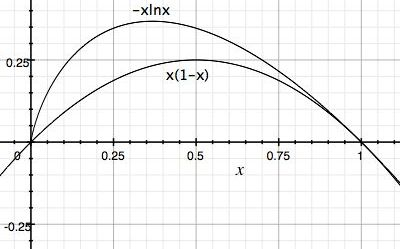
\includegraphics[width=0.6\textwidth]{graph.jpg}
\end{figure}

%------------------------------------------------


\end{document}